% Exemplo de relatório técnico do IC
% Criado por P.J.de Rezende antes do Alvorecer da História.
% Modificado em 97-06-15 e 01-02-26 por J.Stolfi.
% Last edited on 2003-06-07 21:12:18 by stolfi
% modificado em 1o. de outubro de 2008
% modificado em 2012-09-25 para ajustar o pacote UTF8. Contribuicao de
%   Rogerio Cardoso

\documentclass[11pt,twoside]{article}
\usepackage{techrep-PFG-ic}

%%% SE USAR INGLÊS, TROQUE AS ATIVAÇÕES DOS DOIS COMANDOS A SEGUIR:
\usepackage[brazil]{babel}
%% \usepackage[english]{babel}

%%% SE USAR CODIFICAÇÃO LATIN1, TROQUE AS ATIVAÇÕES DOS DOIS COMANDOS A
%%% SEGUIR:
%% \usepackage[latin1]{inputenc}
\usepackage[utf8]{inputenc}
\usepackage{graphicx}
\usepackage{listings}

\begin{document}

%%% PÁGINA DE CAPA %%%%%%%%%%%%%%%%%%%%%%%%%%%%%%%%%%%%%%%%%%%%%%%
% 
% Número do relatório
\TRNumber{01}

% DATA DE PUBLICAÇÃO (PARA A CAPA)
%
\TRYear{18}  % Dois dígitos apenas
\TRMonth{12} % Numérico, 01-12

% LISTA DE AUTORES PARA CAPA (sem afiliações).
\TRAuthor{G. L. da Silva \and E. Borin}

% TÍTULO PARA A CAPA (use \\ para forçar quebras de linha).
\TRTitle{Plataforma de processamento de dados sísmicos como serviço em Nuvem}

\TRMakeCover

%%%%%%%%%%%%%%%%%%%%%%%%%%%%%%%%%%%%%%%%%%%%%%%%%%%%%%%%%%%%%%%%%%%%%%
% O que segue é apenas uma sugestão - sinta-se à vontade para
% usar seu formato predileto, desde que as margens tenham pelo
% menos 25mm nos quatro lados, e o tamanho do fonte seja pelo menos
% 11pt. Certifique-se também de que o título e lista de autores
% estão reproduzidos na íntegra na página 1, a primeira depois da
% página de capa.
%%%%%%%%%%%%%%%%%%%%%%%%%%%%%%%%%%%%%%%%%%%%%%%%%%%%%%%%%%%%%%%%%%%%%%

%%%%%%%%%%%%%%%%%%%%%%%%%%%%%%%%%%%%%%%%%%%%%%%%%%%%%%%%%%%%%%%%%%%%%%
% Nomes de autores ABREVIADOS e titulo ABREVIADO,
% para cabeçalhos em cada página.
%
\markboth{da Silva e Borin}{Processamento sísmico como serviço na nuvem}
\pagestyle{myheadings}

%%%%%%%%%%%%%%%%%%%%%%%%%%%%%%%%%%%%%%%%%%%%%%%%%%%%%%%%%%%%%%%%%%%%%%
% TÍTULO e NOMES DOS AUTORES, completos, para a página 1.
% Use "\\" para quebrar linhas, "\and" para separar autores.
%
\title{Plataforma de processamento de dados sísmicos como serviço em Nuvem}

\author{Guilherme Lucas da Silva \and Edson Borin}

\date{}

\maketitle

%%%%%%%%%%%%%%%%%%%%%%%%%%%%%%%%%%%%%%%%%%%%%%%%%%%%%%%%%%%%%%%%%%%%%%

\begin{abstract} 
  Este trabalho busca criar uma plataforma que facilita o 
  processamento de dados sísmicos na nuvem, sem conhecimento técnico dos
  novos conceitos que a nuvem traz consigo. A partir disso, tenta trazer
  mais agilidade, custos mais baixos e maior flexibilidade para os 
  engenheiros e desenvolvedores que trabalham em aplicações que 
  necessitam de alto poder computacional.

  Desta forma, o projeto foi iniciado com o objetivo de criar uma plataforma
  open source, replicável e extremamente simples de ser usada para qualquer 
  usuário. Os resultados foram muito positivos, alcançando o intuito de criar
  a plataforma somente com componentes open source e facilmente replicável em
  diversas situações.
\end{abstract}

\section{Introducão}

Computação em Nuvem é um conceito que está cada vez mais presente no cotidiano de todas as pessoas. Mesmo sem perceber, uma quantidade gigantesca de aplicações que usamos hoje 
em dia lançam mão desse conceito tão central para o desenvolvimento econômico e tecnológico de nossa sociedade contemporânea. Ela se baseia na capacidade de usarmos o
poder computacional de uma infinidade de serviços como Máquinas virtuais, Bancos de Dados e Redes Virutais sem necessariamente possuirmos máquinas físicas com tais serviços 
instalados e configurados, ainda sendo possível, de maneira simples, expor tais serviços e mecanismos para vários usuários ao redor do mundo. Segundo o artigo Cloud Computing Security: A
Systematic Literature Review~\cite{UPP}, computação em nuvem é um modelo de rede que torna possível o acesso sob demanda de recursos computacionais configuráveis.
Entre as modalidades principais de serviços de computação em nuvem, temos três categorias mais relevantes:

\begin{itemize}

  \item \textbf{IaaS(Infrastructure as a Service):} essa é a maneira que dá mais responsabilidade ao usuário. Essa modalidade te dá máquinas virtualizadas que você deve gerenciar 
  instalação de programas, configurações e etc. Exemplo disso são máquinas virtuais que rodam sistemas operacionais GNU/Linux e são acessadas remotamente.
  \item \textbf{PaaS(Plataform as a Service):} Aqui, o usuário não precisa se preocupar com pacotes de sistema, softwares e configurações. Esse sabor de computação em nuvem, tenta 
  facilitar para desenvolvedores publicarem suas aplicações. Isso siginifca que se, por exemplo, um usuário quiser publicar uma aplicação, não vai precisar se preocupar em
  instalar compiladores nem pacotes necessários para rodar a aplicação naquela determinada linguagem.
  \item \textbf{SaaS(Software as a Service):} essa é a modalidade que traz menos autonomia para o desenvolvedor, sendo que, através dela, todo o rescurso é gerenciado pelo provedor de 
  nuvem que é consumido. Alguns exemplos que podemos citar para ilustrar são bancos de dados como serviço, onde o usuário não se preocupa com nenhum tipo de infraestrutura, 
  somente usa o endereço que o provedor cede e faz uso das possibildiades de armazenamento que a plataforma oferece.

\end{itemize}

Entre as vantagens de se adotar um modelo de computação em nuvem ao invés de investir em adiquirir máquinas físicas, podemos citar:

\begin{itemize}
  \item \textbf{Custo:} devido a possibilidade de pagar somente pelo o que está usando, ou seja, caso algum recurso está sendo pouco aproveitado, basta desligá-lo, usuários desse tipo de 
  plataforma não gastarão para manter sistemas parados.
  \item \textbf{Escalabilidade:} A computação em nuvem permite que, caso a aplicação precise de muito mais poder computacional do que possui no momento, seja extremamente simples aumentar
  o número de instâncias ou o tamanho das máquinas, para atender mais usuários, gerando assim, mais receita.
  \item \textbf{Foco na aplicação:} desenvolvedores podem focar totalmente em escrever suas aplicações, sem a preocupação de gerenciar infraestutura e plataforma, o que pode ser muito
  trabalhoso.

\end{itemize}

Entre os principais players de nuvem pública atualmente temos gigantes como Microsoft Azure\footnote{Plataforma de Computação em Nuvem da Microsoft https://azure.microsoft.com/}, 
Amazon Web Services\footnote{Plataforma de Computação em Nuvem da Amazon https://aws.amazon.com/} e Google Cloud Platform\footnote{Plataforma de Computação em Nuvem do Google https://cloud.google.com/}, 
oferecendo opções extremamente diversas para computação em nuvem, desde máquinas virtuais até mesmo bancos de dados gerenciados, onde a preocupação de gerenciamente fica totalmente
do lado do provedor do serviço.

Aplicações de HPC (High Processing Computing, computação de alto processamento, na tradução) são uma gama de programas que necessitam de muito poder computacional para 
completar seus objetivos. Entre essas tarefas, estão o processamento de dados sísmicos, que são obtidas de maneira bruta e precisam de um trabalho muito pesado de tratamento
para que algumas conclusões possam ser feitas a partir dele. Segundo o texto~\cite{HPC}, Supercomputação é usada para realizar operaçoes matemáticas em alta velocidade. HPC é como supercomputação,
mas com o poder computacional de cluster computacionais.
Ainda hoje, muitas dessas operações são feitas em servidores em institutos de pesquisas, por exemplo, podendo levar
a um custo excessivo, trabalho excessivo para gerenciamento de infraestrutura além de baixíssima agilidade e flexibilidade quanto a infraestrura. Assim, tais aplicações podem 
tirar muito proveito dos provedores de nuvem citados acima.

\section{Objetivos}
Esse trabalho tem como objetivo desenvolver uma plataforma Open Source que torne extremamente simples para usuários que não conhecem conceitos de Computação em Nuvem rodarem suas aplicações.
Entre os princípios do Open Source citado no Debian Social Contract~\cite{BP}: Redistribuição livre, o software deve ser distrivuído com o código fonte, trabalhos derivados, entre outros.
A princípio, foram usadas aplicações sísmicas para a prova de conceito. O desejado para o final da plataforma era que os usuários conseguissem processar 
os trabalhos sísmico sem necessariamente conhecer plataformas de Nuvem.  
Ao final, é esperado a criação de uma plataforma web, que tinha como principais funcionalidades:

\begin{itemize}
  \item \textbf{Submissão e gerenciamente de dados:} Essa funcionalidade é a responsável pelo upload de dados sísmicos que serão usados nos processamentos, além de consultar quais foram submetidos, baixá-los e também
  excluí-los, caso necessário. 
  \item \textbf{Submissão e gerenciamento de binários:} esse componente do projeto é extremamente semelhante com a que detalhamos acima, porém, ao invés dos dados sísmicos, os artefatos que são gerenciados são os 
  binários das aplicações que serão utilizados nos processos.
  \item \textbf{Definição de tarefas sísmicas:} Utilizando os dados e binários submetidos a partir das duas funcionalidades citadas anteriormente, o objetivo era conseguir lançar um processamento que combina os dados e 
  binários, além dos argumentos necessários.
  \item \textbf{Obtenção dos resultados:} Ao final dos processos, é desejado que se consiga obter todos os resultados desse de maneira simples e rápida.
\end{itemize}

\section{Relevância}
Ao buscar por outras soluções que tem o mesmo intuito da plataforma que esse trabalho tem por objetivo desenvolver, notamos a sua extrema relevância, uma que vez que é muito difícil achar outros softwares
open source que executam tal tarefa.
Além da unicidade que o trabalho possui no cenários atual, ele se torna relevante já que ele pode abstrair os novos conceitos e a curva de aprendizado que vem junto com a computação em nuvem. Assim é possível
tirar proveito de todos os benefícios que foram citados acima, levando a possibilidade de um uso muito mais inteligente dos recursos, baixando custos e aumentando a produtividade.

\section{Procedimento}
Para o sucesso do projeto, ao começo dele, foi decidido que faríamos uma plataforma web. Essa foi a decisão devido a facilidade de desenvolver para esse tipo de plataforma, além do alcance
gigantesco que plataformas web possuem, já que é praticamente obrigatório nos dispositivos que os usuários poderiam usar para acessar o sistema (smartphones e computadores) possuir um
navegador de internet instalado. Além disso, vale ressaltar que desde o início do projeto todo o código estava totalmente aberto no Github\footnote{Serviço para compartilhamento de código fonte www.github.com}, 
já que foi uma premissa desde o início do projeto que este seria Open Source.

Ao iniciar a análise do problema, foi possível notar que uma arquitetura de nuvem que se encaixa muito bem nesse problema é a de Work Queues(Filas de Trabalho), que segundo Brendan Burns em seu livro
Designing Distributed Systems, "Em um sistema de filas de trabalho existe uma trabalho em batch para ser executado. Cada parte do trabalho é independente do outro e pode ser executado sem nenhuma interaçao" 
~\cite{BB}.
Isso é exatamente o que foi buscado, uma vez que os trabalhos eram intensivos, demoravam um tempo significativo para serem reproduzidos e eram independentes um do outro. Assim, o que gostaríamos era que trabalhos fossem submetidos
a uma fila e, alguma unidade de computação o usasse para executar uma definição de trabalho.

\begin{figure}[!h]
  \centering
  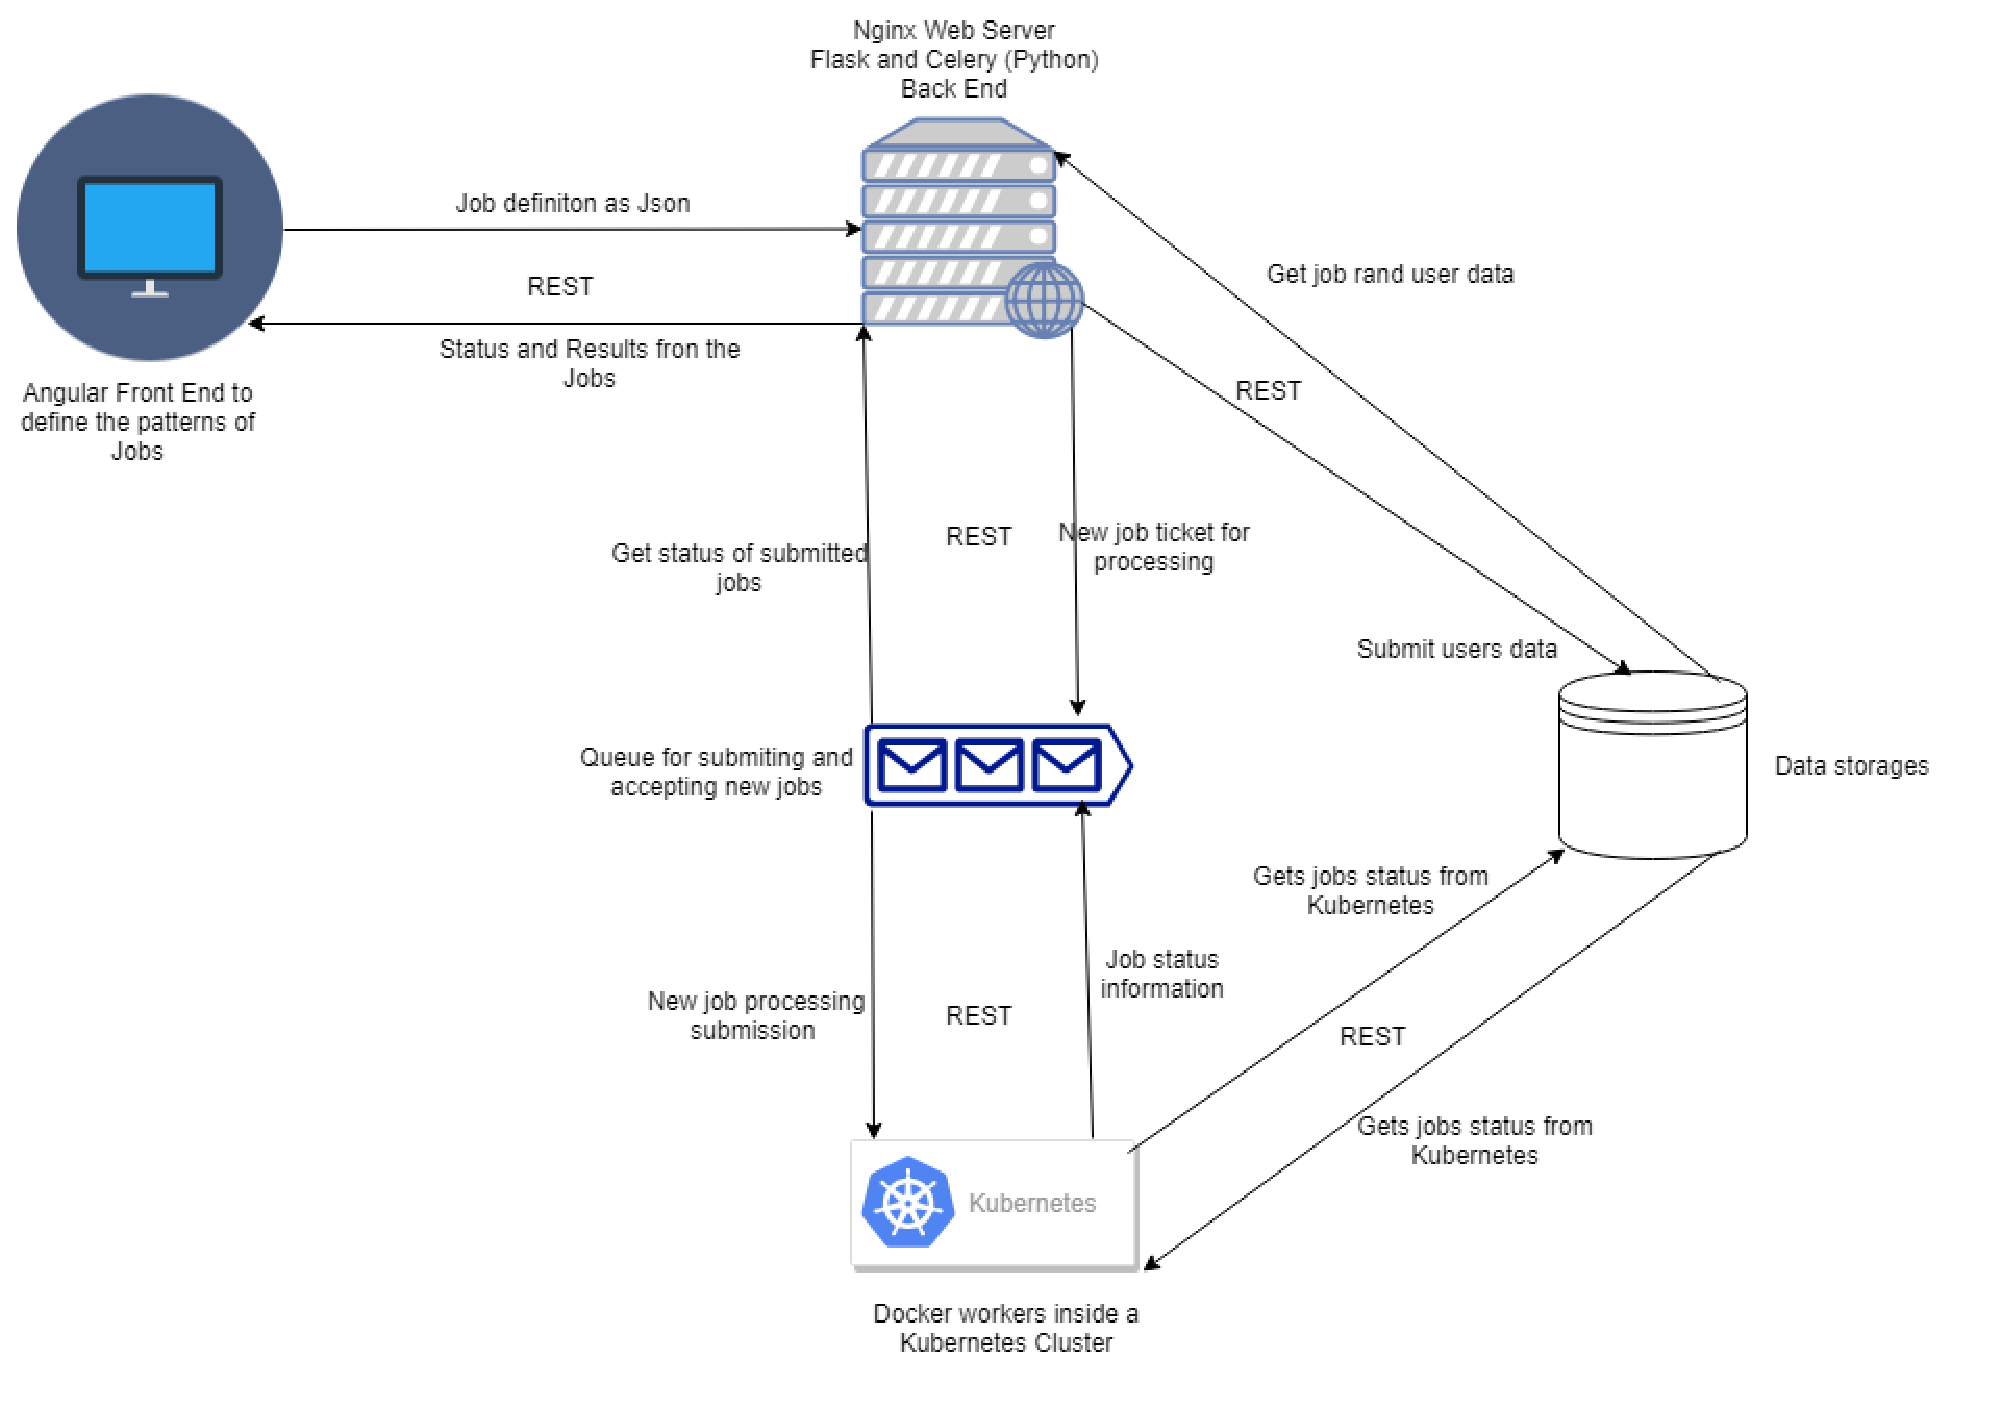
\includegraphics[scale=0.4]{arch.eps}
  \caption{Arquitetura inicial do projeto e exemplo de filas da trabalho distribuídas}
  \label{fig:archtec}
\end{figure}

A imagem ~\ref{fig:archtec} ajuda a explicar como é o funcionamento dessa arquitetura e a arquitetura inicial do projeto.

Então, a plataforma foi separada em duas grandes partes:

\begin{itemize}
  \item \textbf{Front-End:} A parte que o usuário realmente vê, o código que irá rodar no navegador do seu dispositivo. 
  \item \textbf{Back-End:} Essa é a porção da plataforma responsável por características que são invisíveis ao usuário. Entre elas, podemos citar acesso ao banco de dados, autenticação, processamento de dados,
  submissão de dados para a nuvem, etc.
\end{itemize}

Existem alguns componentes que foram usados em comum entre essas duas partes:

\begin{itemize}
  \item \textbf{Docker\footnote{Programa que realiza virtualização em nível de Sistema Operacional, também conhecido como conteinerização https://www.docker.com/}:} 
  uma maneira muito simples de empacotar as aplicações, isolando dependências, garantindo que o deploy sempre é feito da maneira correta. Assim, é possível entregar as aplicações completas, com
  todos os requisitos necessários instalados, o que da uma agilidade enorme durante o ciclo de desenvolvimento.
  \item \textbf{Nginx\footnote{Servidor Web Open Source https://www.nginx.com/}:} Servidor web open source extremamente escalável e fácil de configurar. Foi usado tanto para servir o back end quando o front end. 
  A outra opção para esse trabalho seria o Apache Web Server, porém o Nginx se mostrou mais simples e rápido de ter aplicações rodando.
\end{itemize}

\subsection{Front End}

Para o desenvolvimento do front end, foram definidas de antemão como seria a composição geral das telas e como seria o fluxo da aplicação. Assim, o layout geral das telas, seria:

\begin{figure}[!h]
  \centering
  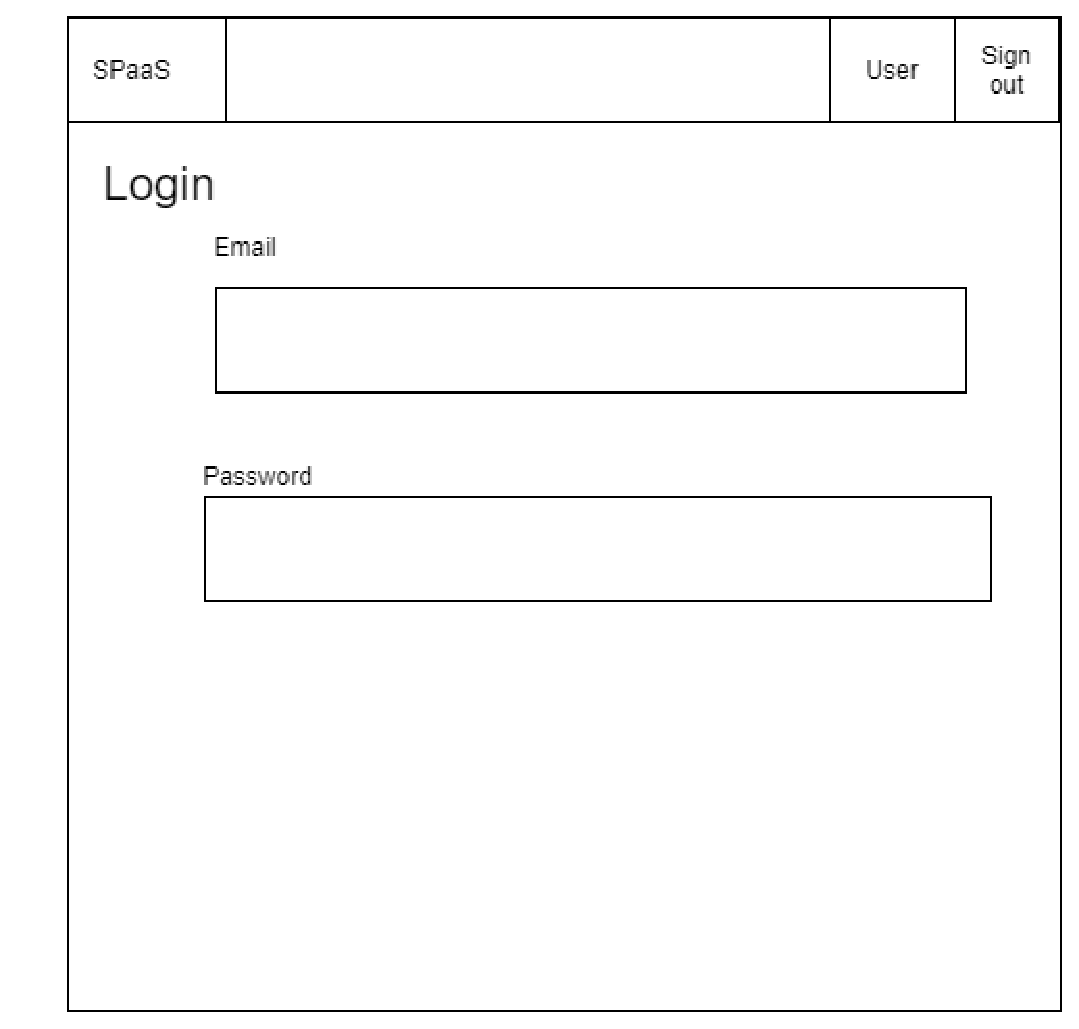
\includegraphics[scale=0.4]{login.eps}
  \caption{Página de Login}
  \label{fig:loginScreen}
\end{figure}

A figura ~\ref{fig:loginScreen} mostra como definimos quais informações deveriam estar na tela para que o usuário pudesse se conectar a plataforma. Como mostrado, 
as informações necessárias para logar no sistema eram email e senha que foram previamente cadastrado.

\begin{figure}[!h]
  \centering
  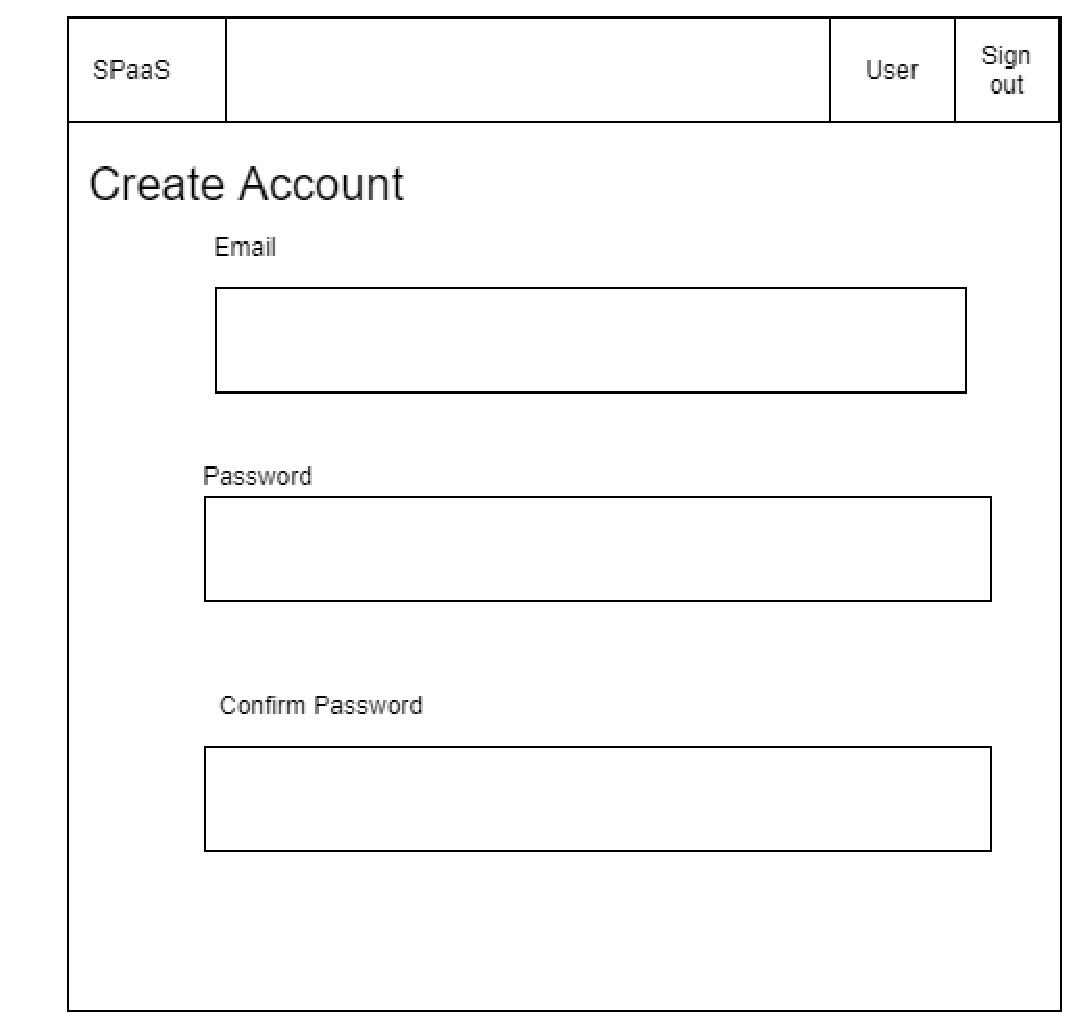
\includegraphics[scale=0.4]{account_reg.eps}
  \caption{Página de criaçao de conta}
  \label{fig:createScreen}
\end{figure}

A figura ~\ref{fig:createScreen} deixa claro quais foram as informações que eram requeridas para se criar uma conta no sistema. 

\begin{figure}[!h]
  \centering
  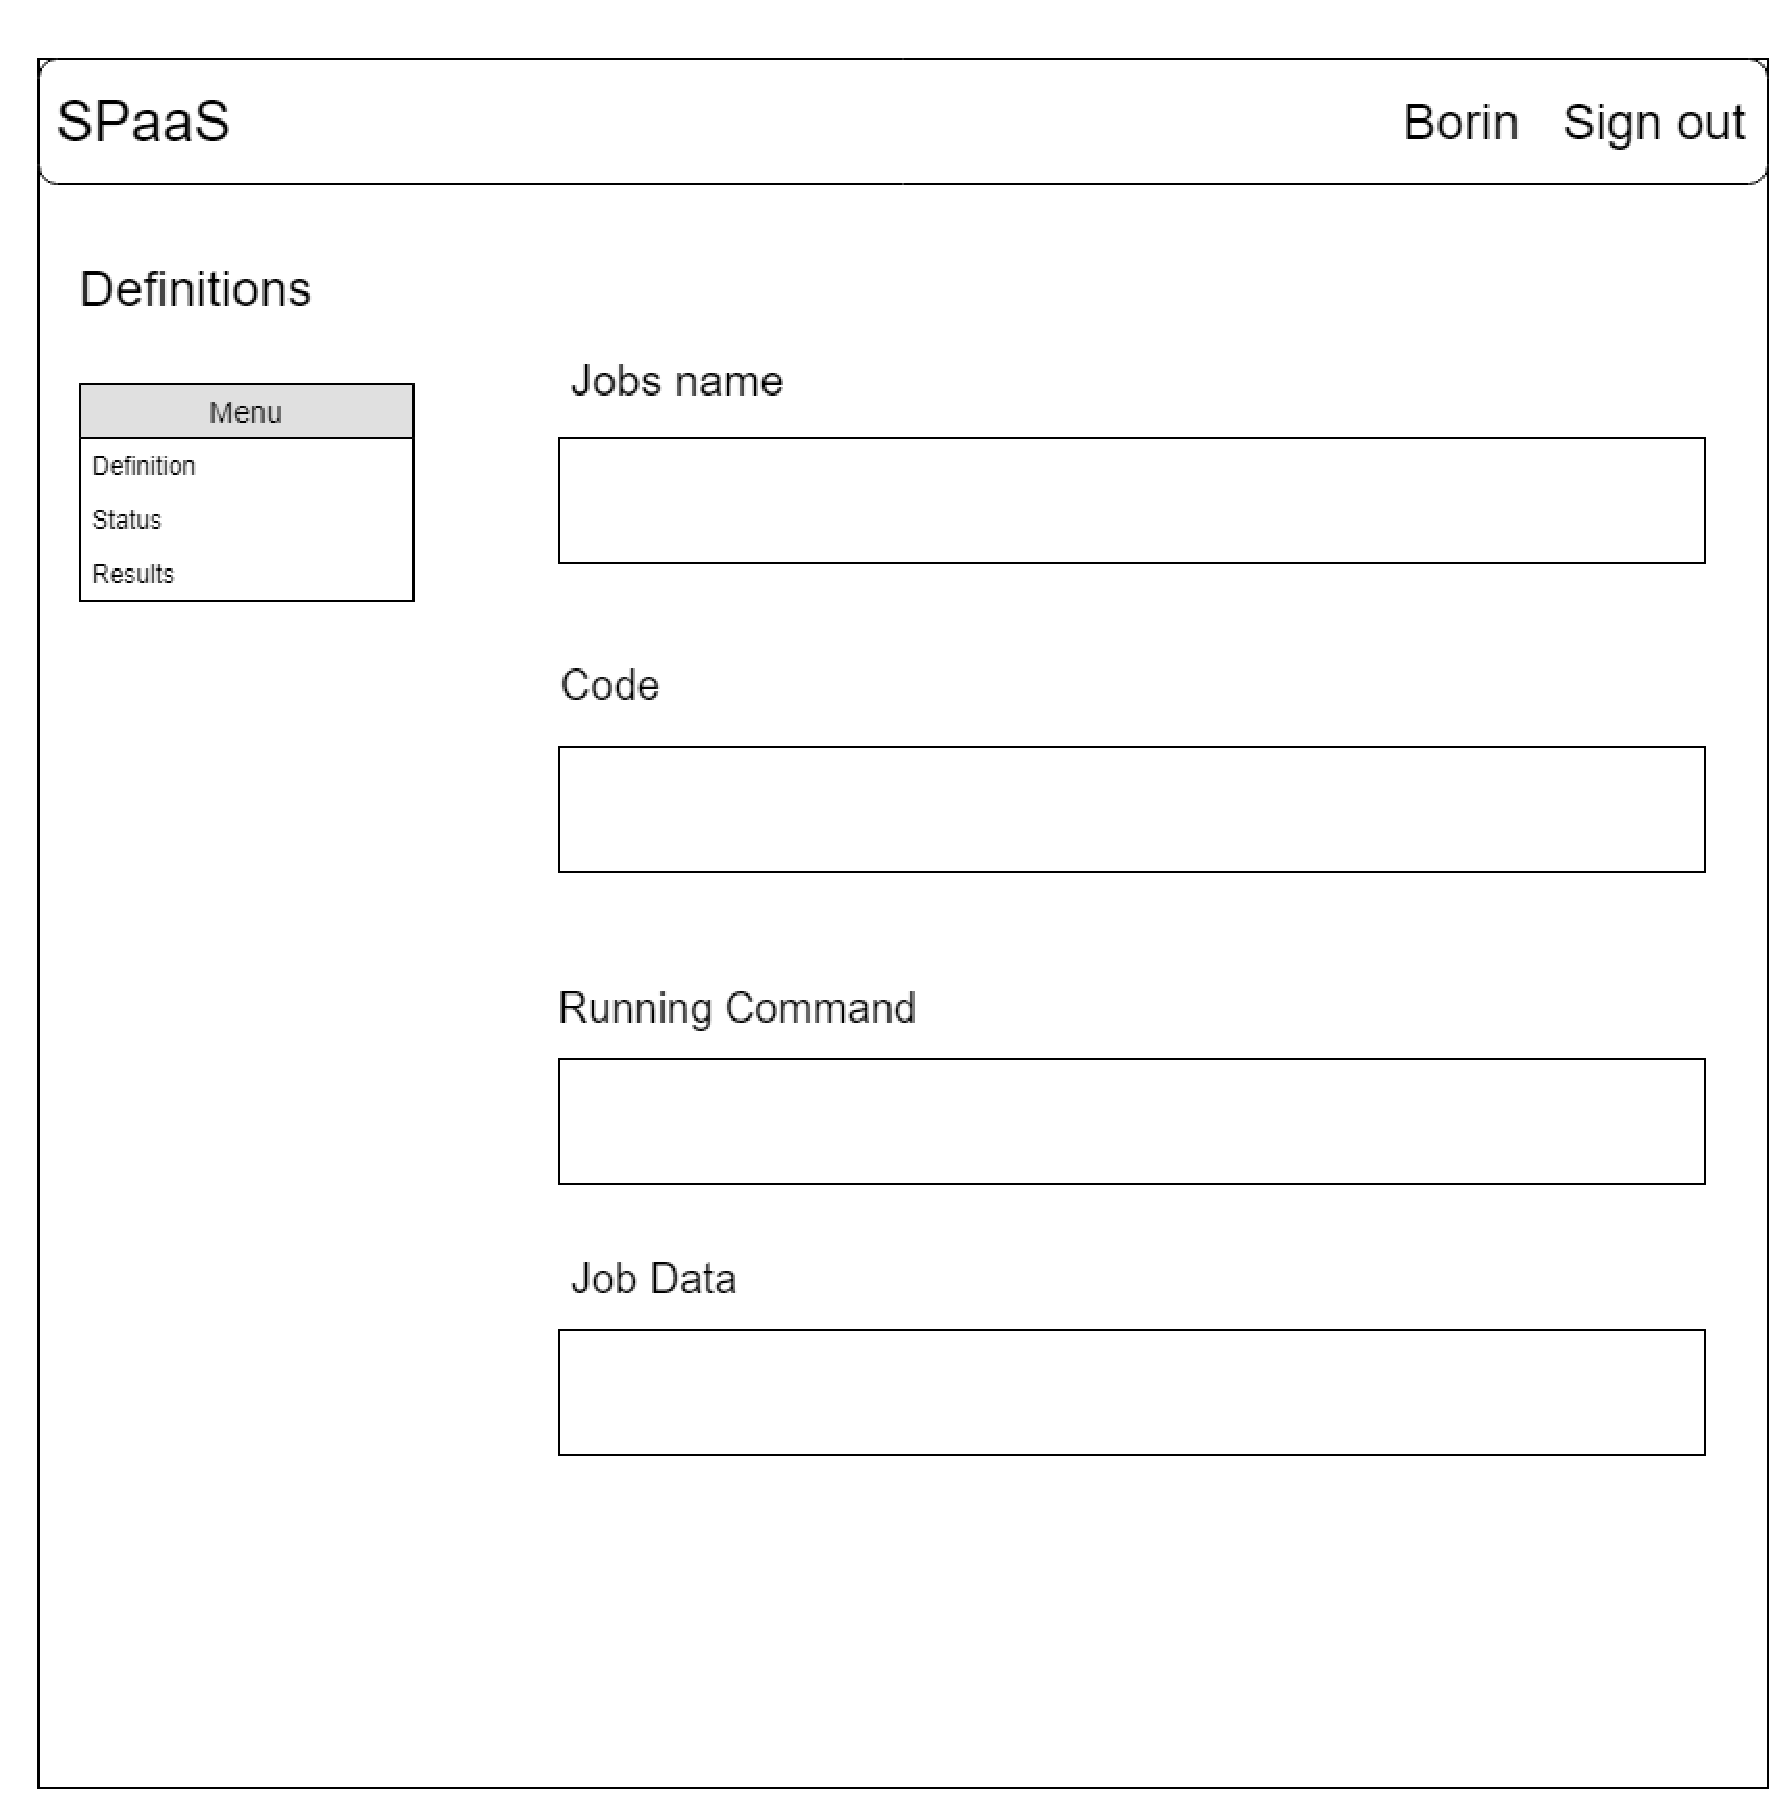
\includegraphics[scale=0.2]{First_screen.eps}
  \caption{Página de definição dos trabalhos}
  \label{fig:definitionScreen}
\end{figure}


A figura ~\ref{fig:definitionScreen} exemplifica como imaginamos a tela de definicao de um trabalho para ser executado. Nesse primeiro protótipo, foi pensado que somente 
as informações mostradas na tela, eram o suficente.

\begin{figure}[!h]
  \centering
  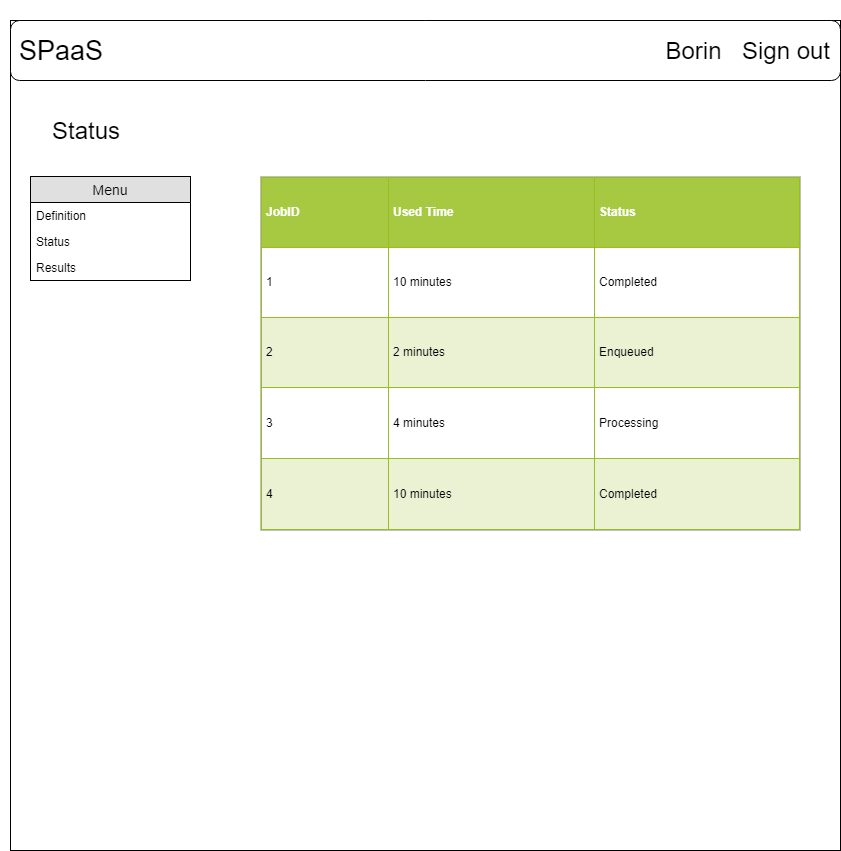
\includegraphics[scale=0.2]{Second_screen.eps}
  \caption{Página de observação do status}
  \label{fig:statusScreen}
\end{figure}


O protótipo da tela de status dos trabalhos está mostrada na figura ~\ref{fig:statusScreen}. Extremamente simples a princípio, uma tabela mostrando o status de cada trabalho. 

\begin{figure}[!h]
  \centering
  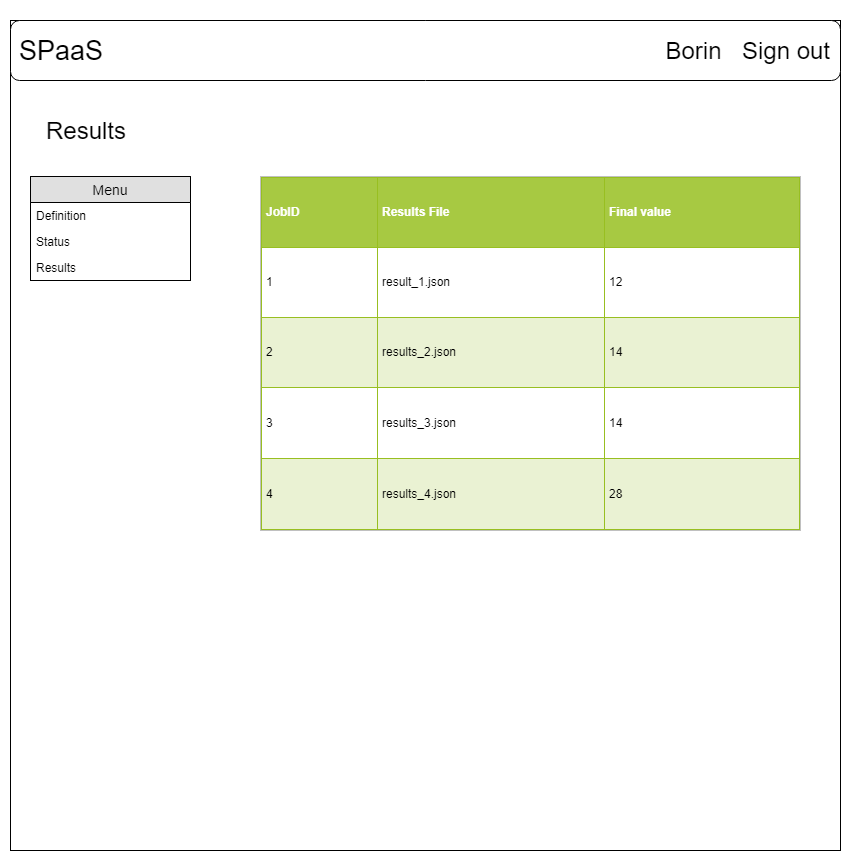
\includegraphics[scale=0.2]{Third_screen.eps}
  \caption{Página de obtenção dos resultados}
  \label{fig:resultsScreen}
\end{figure}

A ultima figura ~\ref{fig:resultScreen} mostra como foi pensada a obtenção dos resultados.

\begin{figure}[!h]
  \centering
  \includegraphics[scale=0.2]{tcc_flow.eps}
  \caption{Fluxo entre os componentes da plataforma}
  \label{fig:flowScreen}
\end{figure}

Vale ressaltar que essa ideia inicial foi considerada com poucas das funcionalidades que realmente eram relevantes para a plataforma. Assim, o fluxo de todo o trabalho foi 
repensado para algo mais próximo do representado na figura ~\ref{fig:flowScreen}. Nesse fluxo definido, os quadrados representam as telas, com suas respectivas interações com 
as camadas de armazenamento, que são necessárias para completar suas tarefas com sucesso. Assim, entrando no detalhe de cada componente da solução:

\begin{itemize}
  \item \textbf{Data Management:} Componente responsável pelo gerencimento dos dados sísmicos da plataforma. A intenção nesse componente é ser capaz de adicionar, remover e 
  movê-los de um tipo de armazenamento mais caro (porém mais rápido) para um mais barato, ligeiramente mais lento. 
  \item \textbf{Flow Management:} Componente responsável por determinar uma sequencia de passos que devem ser feitas para completar uma tarefa. Diferente dos trabalhos (Tasks),
  aqui a definição é de um conjunto de tasks, encadeadas para obter um resultado maior.
  \item \textbf{Tools Management:} Essa funcionalidade procura realizar o gerenciamento dos binários que serão executados. Assim como o componente respoonsável pelo gerenciamento
  dos dados, esse componente busca dar a possibilidade de adicionar, mover e excluir binários da plataforma.
  \item \textbf{Running Tasks:} Nessa tela, é desejado que o usuário consiga ver qual é o status dos processamentos que iniciou. Status como Pendente e Pronto são alguns dos 
  possíveis.
  \item \textbf{New Tasks:} Responsável por definir novas tarefas a serem rodadas. É desejado que as características necessárias para essa definição sejam binário, dado sísmico 
  e argumentos para a execução acontecer com sucesso. 
  \item \textbf{Results:} Os resultados dos processamentos executados estarão aqui, organizados pela execução que o gerou.
\end{itemize}

Como tecnologias para o desenvolvimento da nossa plataforma, especificamente para o front end, foram escolhidas as seguintes tecnologias:

\begin{itemize}
  \item \textbf{Angular\footnote{Framework Open Source para desenvolvimento web https://angular.io/}:} Framework para desenvolvimento de aplicações web Open Source, desenvolvido inicialmente pelo Google e agora também mantido pela comunidade. Usa como linguagem de desenvolvimento o
  Typescript\footnote{Linguagem criada pela Microsoft. Um superset do JavaScript https://www.typescriptlang.org/}. A escolha desse framework aconteceu uma vez que ele é extremamente produtive e por ser um framework completo, já encapsulando todo o conceito de serviços, estilo de página e 
  linguagem de marcação, roteamento. Assim, com esse framework ainda é necessário conhecer linguagens de marcação como HTML e CSS, mas a junção de todos esses conceitos fica muito mais simples.
  \item \textbf{Bootstrap\footnote{Conjunto de ferramentas Open Source que ajuda na estilização de páginas https://getbootstrap.com/}:} Frameworks que possui o estilo de vários componentes web prontos, como tabelas, menus laterais, barras superiores, etc. É o que muitos sites usam hoje em dia, como é o caso do github
  Estilizar páginas web pode ser um trabalho extremamente complicado e demorado, por isso optamos por usar um framework. Existem outros frameworks CSS interessantes, porém poucos tem a maturidade do bootstrap.
\end{itemize}

Foi garantido que o deploy fosse feito da maneira mais simples e flexível para o cliente. Então, foi usado o servidor web Nginx para isso. Aém disso, também foi disponibilizado um Dockerfile, que possibilita
o deploy da solução de maneira extremamente simples e direta sobre Containers Docker.

\subsection{Back End}

Ao início do desenvolvimento do back end, buscamos definir quais seriam as melhores tecnologias para esse componente, além de definir como seriam as rotas e contratos que a API do back end iria expor
para que o front end pudesse consumir de forma eficaz e direta, garantindo assim, um total desacoplamento entre os dois componentes. Assim, os componentes que decidimos para o back end foram os seguintes:

\begin{itemize}
  \item \textbf{Python\footnote{https://www.python.org/}:} Linguagem criada por Guido Van Rossum, extremamente relevante nos dias de hoje devido a sua enorme gama de aplicações, que vão desde embarcados até sistemas de análise de dados de alto 
  desempenho. A escolha dela foi devido principalmente a bibliotecas muito maduras para desenvolvimento de API's back end, filas de trabalho distribuídas e conectores com bancos de dados.

  \item \textbf{Flask\footnote{Framework Web Open Source para Python http://flask.pocoo.org/}:} Framework para desenvolvimento de APIS para Python. Foi escolhido devido a extrema agilidade para colocar uma API rodando. Além disso, é muito simples entender como a aplicação está funcionando,
  fator muito crítico para decidirmos na escolha desta, uma vez que o projeto tem como premissa ser Open Source e facilitar o entendimento de todos que o usam. Ao invés de Python/Flask, foram cogitadas também ASP.NET
  com C\# e NodeJS. A primeira foi descartada devido a complexidade para simplesmente criarmos uma API. NodeJS não foi escolhido devido a dificuldade que novos programadores podem enfrentar para compreender as
  fucnionalidades em um primeiro momento, quando fossem aumentar o projeto.

  \item \textbf{Celery\footnote{Framework Open Source para tarefas distribuídas em Python http://www.celeryproject.org/}:} Uma vez escolhido Python e Flask como ferramentas para o desenvolvimento da solução, foi muito natural a escolha do Celery como ferramenta para trabalhar com filas de trabalho. Existem muitos
  casos de sucesso espalhados pela internet de engenheiros e desenvolvedores que usaram essa combinação com total eficácia. O Celery é um componente do Python que é o responsável por gerenciar, submeter e obter
  resultados de uma fila de trabalho, de uma maneira muito simples. Além disso, dá suporte a vários componentes de mensageria, como por exemplo, RabbitMQ\footnote{Plataforma Open Source de Mensageria https://www.rabbitmq.com/}, 
  Redis, Amazon SQS\footnote{Sistema de mensageria da plataforma de AWS https://aws.amazon.com/sqs/}.

  \item \textbf{Redis\footnote{Armazenamento de dados em memória Open Source https://redis.io/}:} Após a escolha de qual biblioteca iríamos usar para facilitar a tarefa de filas de trabalho, que foi o Celery, foi preciso escolher algum componente para a mensageria do projeto, ou seja, o
  componente que realmente é responsável por armazenar e distribuir as mensagens relacionadas aos trabalhos submetidos na solução. Entre as opções estavam RabbitMQ, Redis e Amazon SQS. Essas são as que melhor se 
  integravam com o celery, sendo possível obter todas as suas funcionalidades com qualquer um desses três. Porém, Amazon SQS é uma opção presa a um provedor de nuvem, o que complica o andar do projeto, caso seja 
  preciso usar outra cloud diferente da AWS. RabbitMQ e Redis ofereciam funcionalidades muito parecidas, porém o Redis foi escolhido, devido a infinidade de materiais sobre o uso dele e suas outras funcionalidades
  que podem ser tiradas proveito também, como, por exemplo, cache e armazenamento de dados em memória.

  \item \textbf{MongoDB\footnote{Banco de Dados NoSQL Open Source https://www.mongodb.com/}:} Para o armazenamento dos dados de cadastro de usuários, informações sobre argumentos de cada tipo de binário e etc, a escolha foi um banco de dados NoSQ, o MongoDB. A escolha deste
  foi muito direta, uma vez que os dados que estavam trafegando entre um serviço e outro tinham uma estrutura muito parecida com os documentos que são guardados nesse tipo de banco, não sendo necessário se preocupar
  em transformar os dados para os esquemas presentes em tabelas SQL, o que agiliza muito o trabalho.

  \item \textbf{Blob Storage\footnote{Armazenamento de caráter genérico no Microsoft Azure https://azure.microsoft.com/en-us/services/storage/blobs/}:} o Blob Storage do Microsoft Azure foi a opção aqui pois era necessário uma espécie de armazenamento de propósito geral. Aqui ele está sendo usado para armazenamento dos dados sísmicos e
  binários. Foi escolhido devido a excelente integração que possui com Python. Outras opções existentes eram, por exemplo, Amazon S3 \footnote{Armazenamento genérico na AWS https://aws.amazon.com/pt/s3/}, que oferece serviços muito parecidos. Outra opção era deixar esses dados em 
  no disco de máquinas virtuais e serví-los por meio de servidores, porém, isso aumentaria muito a complexidade e dificultaria a tarefa de gerenciar esse tipo de infraestrutura.
\end{itemize}

\subsection{Ferramentas para Deploy}

Como dito anteriormente, ao iniciar o projeto, não era desejado que estivéssemos presos a um modelo específico de deployment. Assim, para facilitar o deploy da aplicação independente
do modo que foi escolhido para isso, foi criado uma série de scripts em ferramentas específicas para ajudar. Existem dois modelos que estão sendo facilitados:

\begin{itemize}
  \item \textbf{Kubernetes\footnote{Orquestrador de Containers Open Source https://kubernetes.io/}:} Orquestrador de Containers extremamente famoso nos dias de hoje, que tem como principal funcionalidade tornar mais simples, escalável e performática o deploy 
  de aplicações baseadas em Containers. Nascida dentro do Google, a partir do Borg, que segundo o paper pulbicado pelo Google~\cite{BORG}, é um gerenciador de cluster que roda centenas de milhares de processamentos,
  de milhares de diferentes aplicações entre uma série de clusters,
  atualmente está sob a jurisdição da Cloud Native Computing Foundation\footnote{Cloud Native Computing Foundation https://www.cncf.io/} e é Open Source. Foi uma
  das plataformas que foi visada por ter apresentado extremamente relevancia nos ultimos tempos, com todos os grandes provedores de Nuvem oferecendo opções gerenciadas dessa 
  ferramenta.
  \item \textbf{Ansible\footnote{Gerenciador de configuração Open Source https://www.ansible.com/}:} um modelo muito comum de deploy de aplicações é baseada em máquinas virtuais. Nesse caso, é bom garantir que todas as dependências necessárias para que a 
  aplicação rode com sucesso estejam instaladas. Nesse aspecto, o Ansible se mostra extremamente eficaz. Essa ferramenta surgiu da Red Hat e também é mantida Open Souce, sendo um
  ótimo gerenciador de configurações, que torna possível escrever configurações como código, o que garante que a aplicação sempre terá sucesso para ser executada.
\end{itemize}

\section{Resultados}

\subsection{Arquitetura}

\begin{figure}[!h]
  \centering
  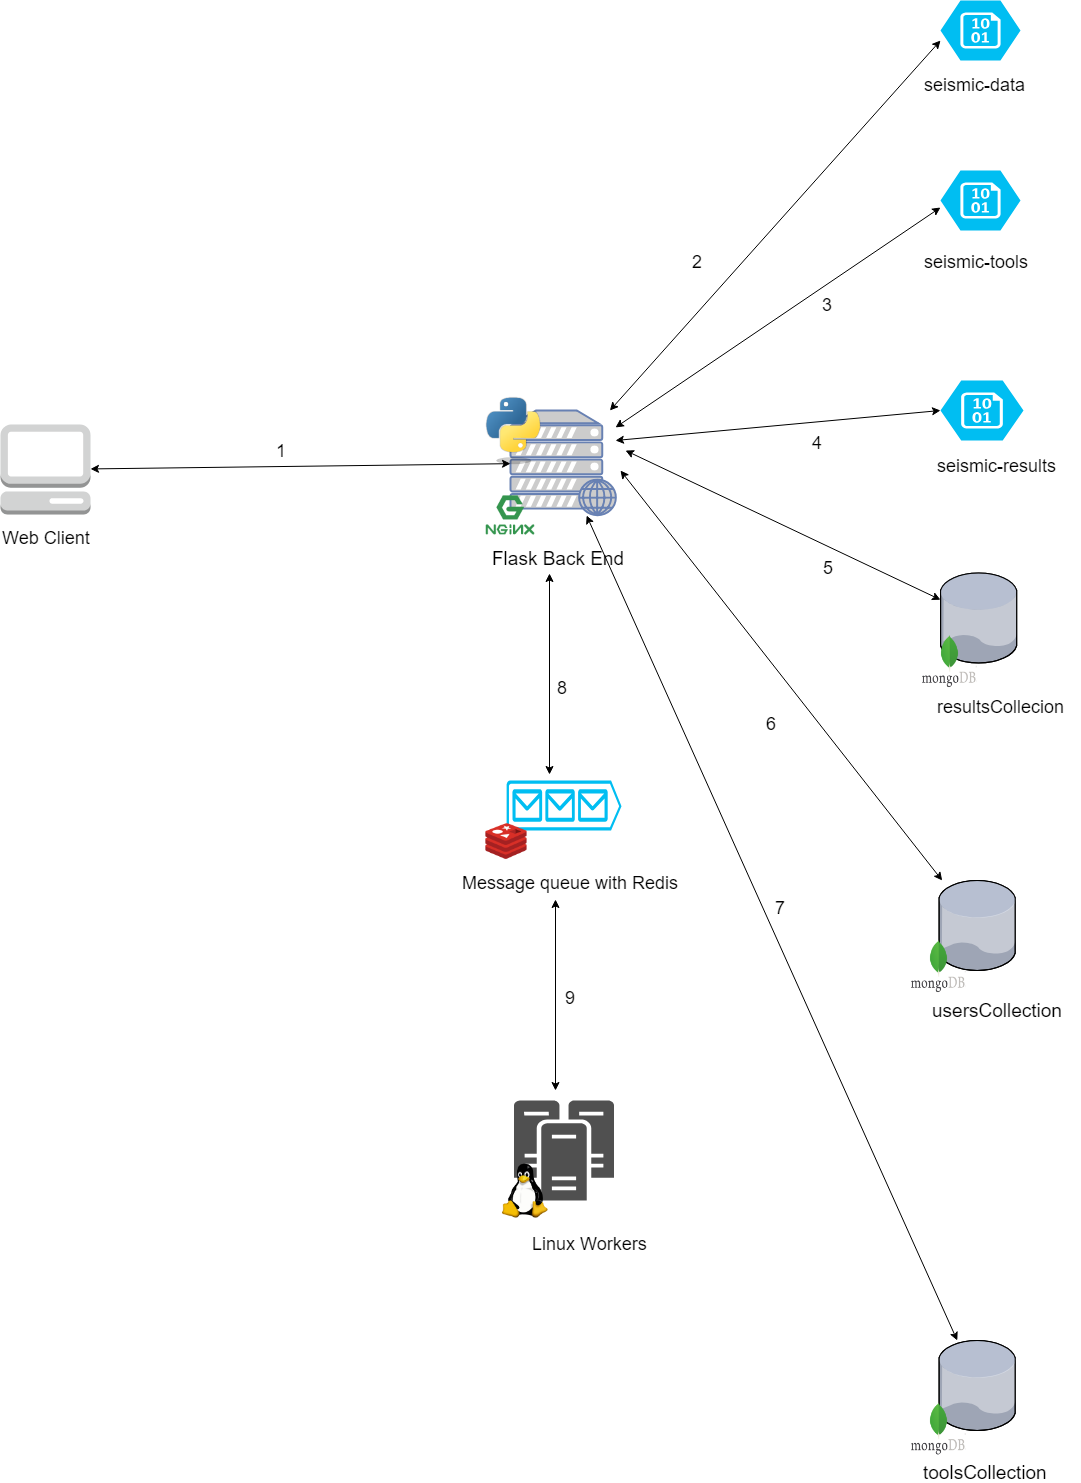
\includegraphics[scale=0.2]{final_arch.eps}
  \caption{Arquitetura final do projeto}
  \label{fig:finalArch}
\end{figure}

Após seguir todo o experimento citado acima, foi alcançado um resultado muito próximo do esperado. A arquitetura final do projeto, está mostrada na figura ~\ref{fig:finalArch}.

Dada a arquitetura final do projeto mostra na figura ~\ref{fig:finalArch} os componentes mostrados tem, cada um, a seguinte função:

\begin{itemize}
  \item \textbf{Web Client:} componete que roda no lado do cliente. Seguimos com o que foi proposto no início do projeto e explicado durante o procedimento, ou seja, todo o código do lado do cliente 
  foi escrito em Typescript, com o auxílio do framework Angular, a estilização das páginas foi feita com Bootstrap e servido via Nginx.
  \item \textbf{Flask Back End:} responsável por receber todas as requisições que saem do front end. Funciona como um gateway. Também foi seguido o plano inicial de escrever todo o back end com
  Python, Flask e Celery. Esse é o componente que possui mais responsabilidades: autenticação, comunicação com a fila com o auxílio do Celery, acesso aos Blobs e acesso ao banco.
  \item \textbf{Linux Workers:} Componente que é responsável pela execução propriamente dita dos pedidos de trabalho. Com o auxílio do Celery, espera por pedidos entrarem na fila, e assim que isso acontece, executam. 
  É possível ter um cluster de máquinas com esse papel, aumentando o paralelismo das execuções.
  \item \textbf{Message queue with Redis:} também parte do plano inicial, a fila de mensagens com o Redis foi a maneira mais eficaz e resiliente que encontramaos de desacoplar o back end dos Linux workers. Assim
  O back end somente precisava submeter uma mensagem com as definições para a execução de um trabalho na fila e algum worker pegaria essa requisição e faria o processamento necessário. Aqui vale um observação 
  importante: A escolha do Celery e do modelo de filas de trabalhos distribuídas, que já foi explicada anteriormente, torna possível, além de desacoplar o back end dos workers, a execução de
  processamentos em paralelo e distribuídos, não criando um gargalo na solução, possivelmente ocasionado pelo grande número de pedidos na fila esperando por um único worker.
  
  \begin{figure}[!h]
    \centering
    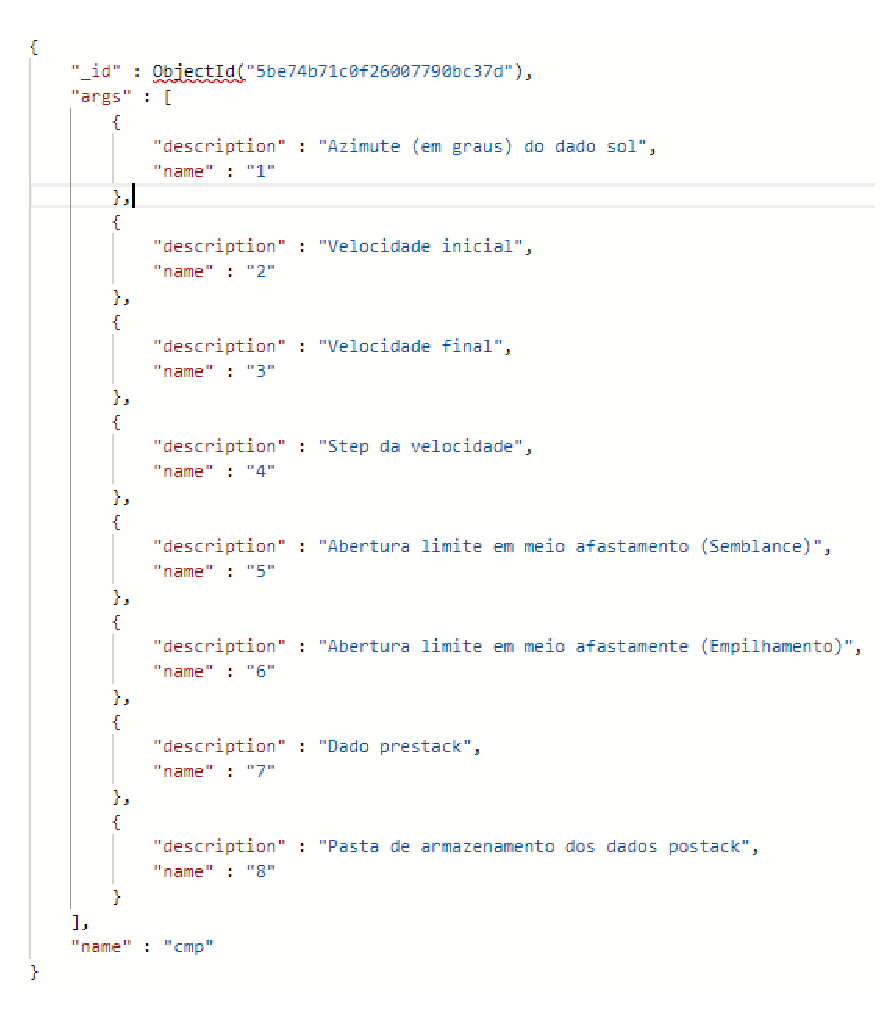
\includegraphics[scale=0.5]{tools_model.eps}
    \caption{Modelo presente na coleção de ferramentas binárias}
    \label{fig:toolsCollection}
  \end{figure}

  \item \textbf{toolsCollection:} coleção dentro do banco que guarda informações sobre os binários que estão armazenados. Novos dados são inseridos nela quando submetidos um novo binário é armazenado, quando
  um novo pedido de processamento será incluído, já que é necessário consultar quais os parâmetros para esse e também quando um binário é excluido, apagando o registro.
  O modelo que está sendo usado para guardar essas informações é o que esta na figura ~\ref{fig:toolsCollection}
  
  \begin{figure}[!h]
    \centering
    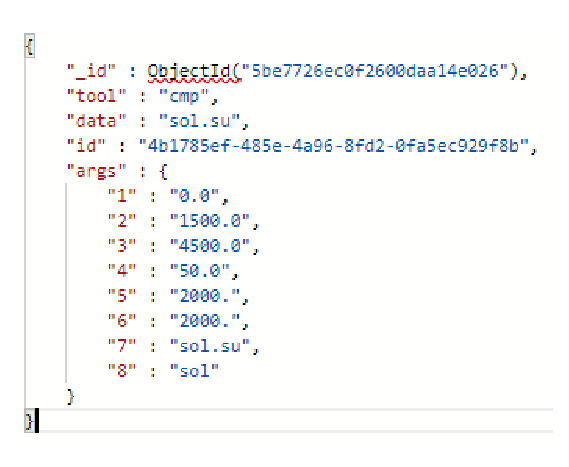
\includegraphics[scale=0.5]{results.eps}
    \caption{Modelo presente na coleção de resultados}
    \label{fig:resultsCollection}
  \end{figure}

  \item \textbf{resultsColleciton:} coleção de documentos no banco para guardar os dados do resultado, armazena o id do processamento, dado e binário usado, além dos argumentos. 
  Essa coleção é acessada após o término de cada processamento, para salvar as informações do resultado e também quando é desejado que todos os resultados sejam mostrados na tela de gerenciamento
  de resultados. O modelo segue o padrão da figura ~\ref{fig:resultsCollection}.

  \begin{figure}[!h]
    \centering
    
\includegraphics[scale=0.5]{users_model.eps}
    \caption{Modelo presente da coleçao de usuários}
    \label{fig:usersCollection}
  \end{figure}

  \item \textbf{usersCollection:} usada para armazenamento de dados dos usuários, como senha e email para autenticação. Um novo registro é criado nessa coleção quando um usuário cria uma nova conta. 
  A coleção também é acessada para autenticação de um novo usuário. Para que todos esses processos sejam executados com sucesso, o modelo usado é o da figura ~\ref{fig:usersCollection}.

  \item \textbf{seismic-tools:} Blob usado para armazenar os binários submetidos pelos usuário. Acessado pelo componemte de gerenciamento de ferramentas quando uma nova ferramente é inserida na plataforma 
  e quando o processamento vai acontecer, pois nesse momento é necessário baixar esses dados para execução em um dos workers.
  \item \textbf{seismic-data:} Blob que armazena os dados sísmicos submetidos. Também são acessados pelo componente de gerenciamento de dados quando um novo dado é incluido, excluído e na execução dos 
  trabalhos, já que é necessário baixar esses dados.
  \item \textbf{seismic-results:} Outro blob. Esse, responsável por armazenar os resultados dos processamentos. Todos os resultados são empacotados em um arquivo tar.gz\footnote{https://www.gzip.org/} e disponibilizados para download, 
  no componente responsável por gerenciar os resultados.
\end{itemize}

Vale notar aqui que, usamos somente uma instância de bancos de dados, com coleções diferentes para cada tipo de aplicação, as Collections, no caso. Também usamos a mesma estratégia para o blob. Foi usada somente 
uma conta de armazenamento no Microsoft Azure, com pastas separadas para cada uso, que no caso, são seismic-data, seismic-tools e seismic-results. 

\subsection{Rodando a aplicação}

Esta seção é dedicada a explicação de como executar cada componente da plataforma:

\subsubsection{Front End}

Para rodar o front end, todas as variáveis de ambiente estão no caminho front-end/src/environments. Nesse caminho exitem dois arquivos, environment.ts e environment.prod.ts.
O primeiro contém os valores das variáveis de ambiente que serão consideradas durante o desenvolvimento, ou seja, quando o comando

\begin{lstlisting}[language=bash]
  $ ng serve 
\end{lstlisting}

é usado. Assim, a única variável que deve ser alterada é a apiUrl, que deve apontar para o back end. Assim para compilar o projeto e serví-lo usando um servidor web, os comandos que 
devem ser rodados são os seguintes: 

\begin{lstlisting}[language=bash]
  $ npm install 
  $ npm run build -- --output-path=./dist/out --configuration production
\end{lstlisting}

Isso gerará uma pasta ./dist/out que quando colocadas no caminho /usr/share/nginx/html de um computador com nginx instalado, irá servir a aplicação do front end.

Outra maneira de rodar o front end é via docker. Existe um Dockerfile dentro da pasta front end que facilita muito o deploy. Existem dois comandos que devem ser rodados nesse caso, um
para construir a imagem do Docker e outro para rodá-la:

\begin{lstlisting}[language=bash]
  $ docker build -t my-angular-project:prod .
  $ docker run -p 80:80 my-angular-project:prod
\end{lstlisting}

Ao acessar o localhost, será possível ver a tela inicial do projeto.

\subsubsection{Back End}

Aqui, assim como no front end, também existe a possibilidade de rodar o código nativamente ou dentro de um container Docker. Para rodar o back end nativamente, dentro da pasta back end
existe o arquivo main.py e o requirements.txt. O arquivo de requirements.txt mostra quais são os pacotes necessários para rodar a aplicação. Além desses dois arquivos, é preciso definir três
variáveis de ambiente, que são:

\begin{itemize}
  \item SPASS\_CONNECTION\_STRING: String de conexão do MongoDB que será usado para a aplicação.
  \item SPASS\_DATA\_BLOB\_KEY: Chave referente ao blob que irá guardar todos os componentes citados anteriormente: resultados, dados e binários.
  \item SPASS\_CELERY\_BROKER: String de conexão do broker do Celery, que, no caso do nosso experimento é o Redis.
\end{itemize}

Assim, após adicionar essas variáveis de ambiente, basta, dentro da pasta back end, rodar os seguintes comandos:

\begin{lstlisting}[language=bash]
  $ pip3 install -r requirements.txt
  $ python3 main.py
\end{lstlisting}

Caso a opção seja por rodar o back end com Docker, os comandos são:

\begin{lstlisting}[language=bash]
  $ docker build -t flask-back .
  $ docker run -p 5000:5000 -e SPASS\_CONNECTION\_STRING="<value>" -e SPASS\_DATA\_BLOB\_KEY="<value>" -e SPASS\_CELERY\_BROKER="<value>" flask-back
\end{lstlisting}

Nesse caso, o back end estará escutando na porta 5000.

\subsubsection{Worker}

Para os workers, também é possível rodá-lo nativamente. Para isso, dentro da pasta back end, basta executar:

\begin{lstlisting}[language=bash]
  $ pip3 install -r requirements.txt
  $ celery worker -A main.celery -l info
\end{lstlisting}

Vale lembrar que nos workers também é necessário declarar as mesmas variáveis de ambiente do back end, citadas anteriormente. 
Porém, como a proposta é ter vários workers para executar as tarefas em paralelo, foi criado um playbook Ansible, para configurar deixar várias máquinas prontas para 
executar essas tarefas. Para isso, com o Ansible instalado e os hosts determinado no arquivo de configuração da ferramenta, basta executar dentro da pasta devops:

\begin{lstlisting}[language=bash]
  $ ansible-playbook worker_config.yaml
\end{lstlisting}

\subsection{Telas finais}

Assim, após apresentar a arquitetura final, são apresentadas os componentes, com suas respectivas telas. 

\begin{figure}[!h]
  \centering
  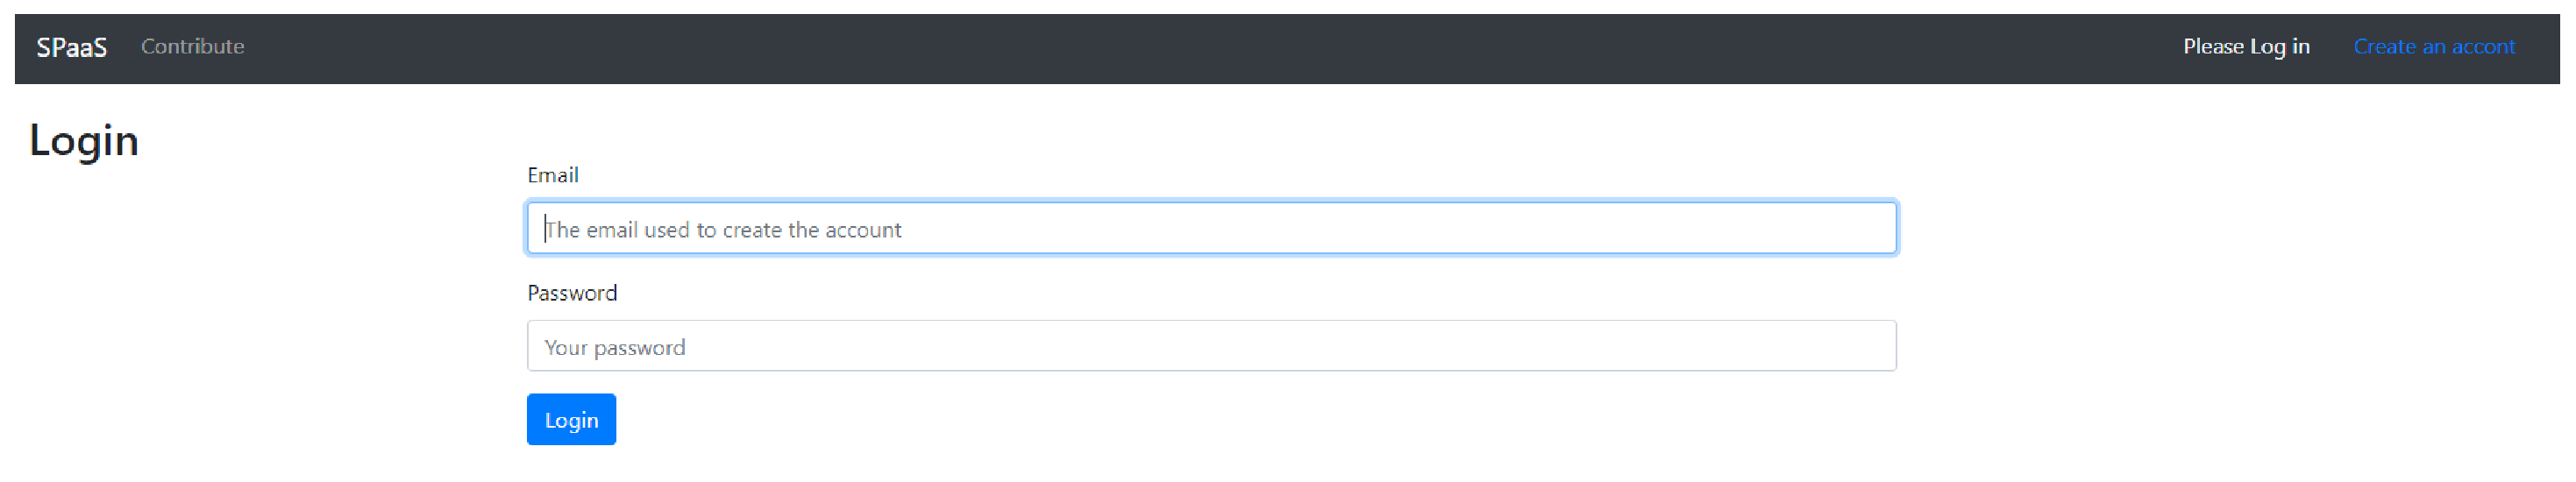
\includegraphics[scale=0.3]{final_login.eps}
  \caption{Tela final do login}
  \label{fig:finalLogin}
\end{figure}

Na tela final de login, figura ~\ref{fig:finalLogin}, existe dois campos muito simples e comuns em sites que necessitam autenticação: email e senha. Além disso, caso você não possua uma conta, é possível criar uma no canto superior direito.

\begin{figure}[!h]
  \centering
  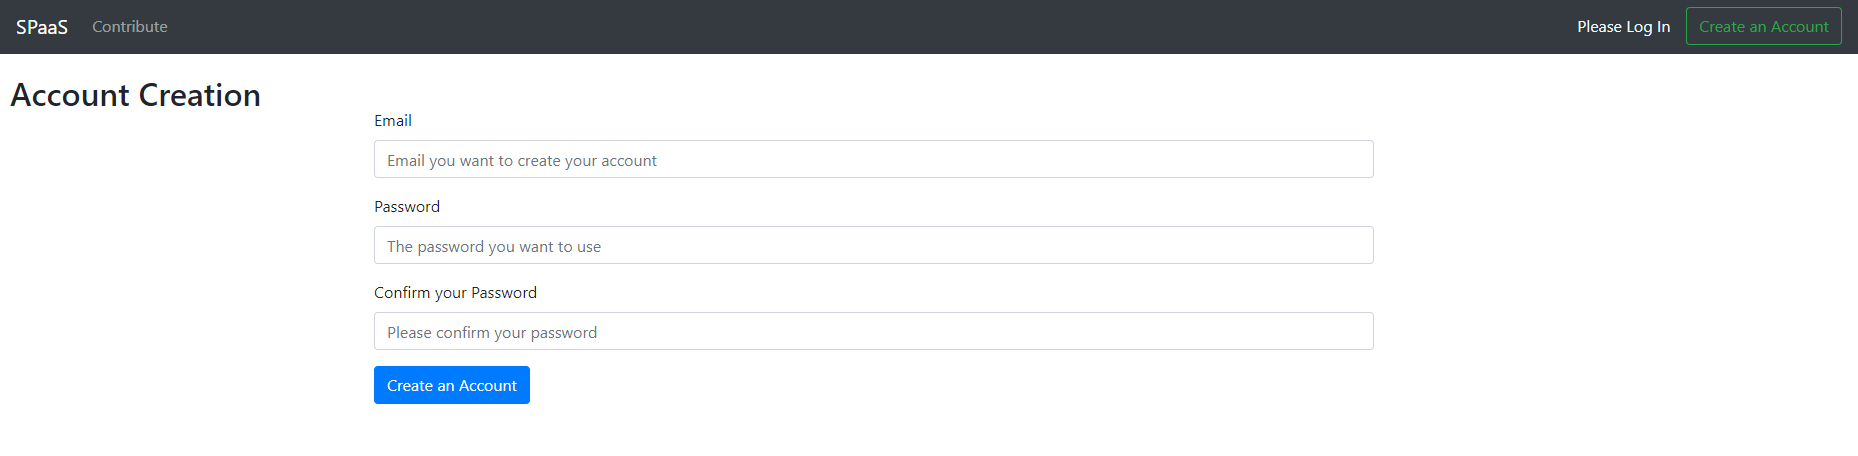
\includegraphics[scale=0.3]{final_create.eps}
  \caption{Tela final de criação de contas}
  \label{fig:finalCreate}
\end{figure}

Caso, na tela de login, for escolhido a tela que o usuário será direcionado é a ~\ref{fig:finalCreate}, onde será possível criar uma nova conta com email e senha, que deve ser confirmada. Aqui, existe a verificação
se o email já foi usado, para garantir que cada usuário só tenha uma conta cadastrada.

\begin{figure}[!h]
  \centering
  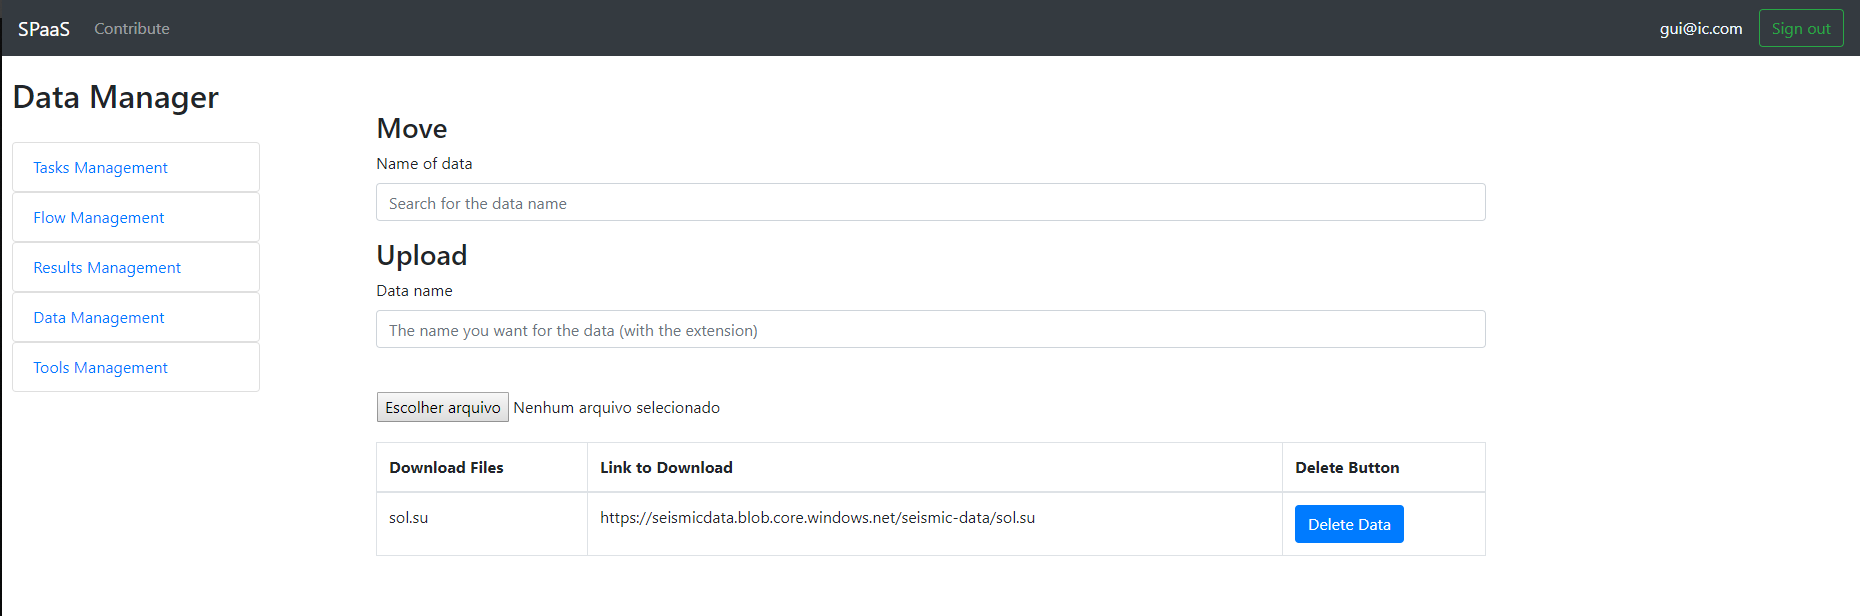
\includegraphics[scale=0.3]{data_final.eps}
  \caption{Tela final de gerenciamento de dados sísmicos}
  \label{fig:finalData}
\end{figure}

Na imagem ~\ref{fig:finalData} é possível observar como todas as funcionalidades que foram planejadas no início estão sendo contempladas. Na seção de Upload, é possível definir um nome para o dado, e escolher o 
arquivo que será submetido. Além disso, a tabela abaixo mostra todos os dados que foram submetidos, com o link para download e também a opção de deletar os já existentes.

\begin{figure}[!h]
  \centering
  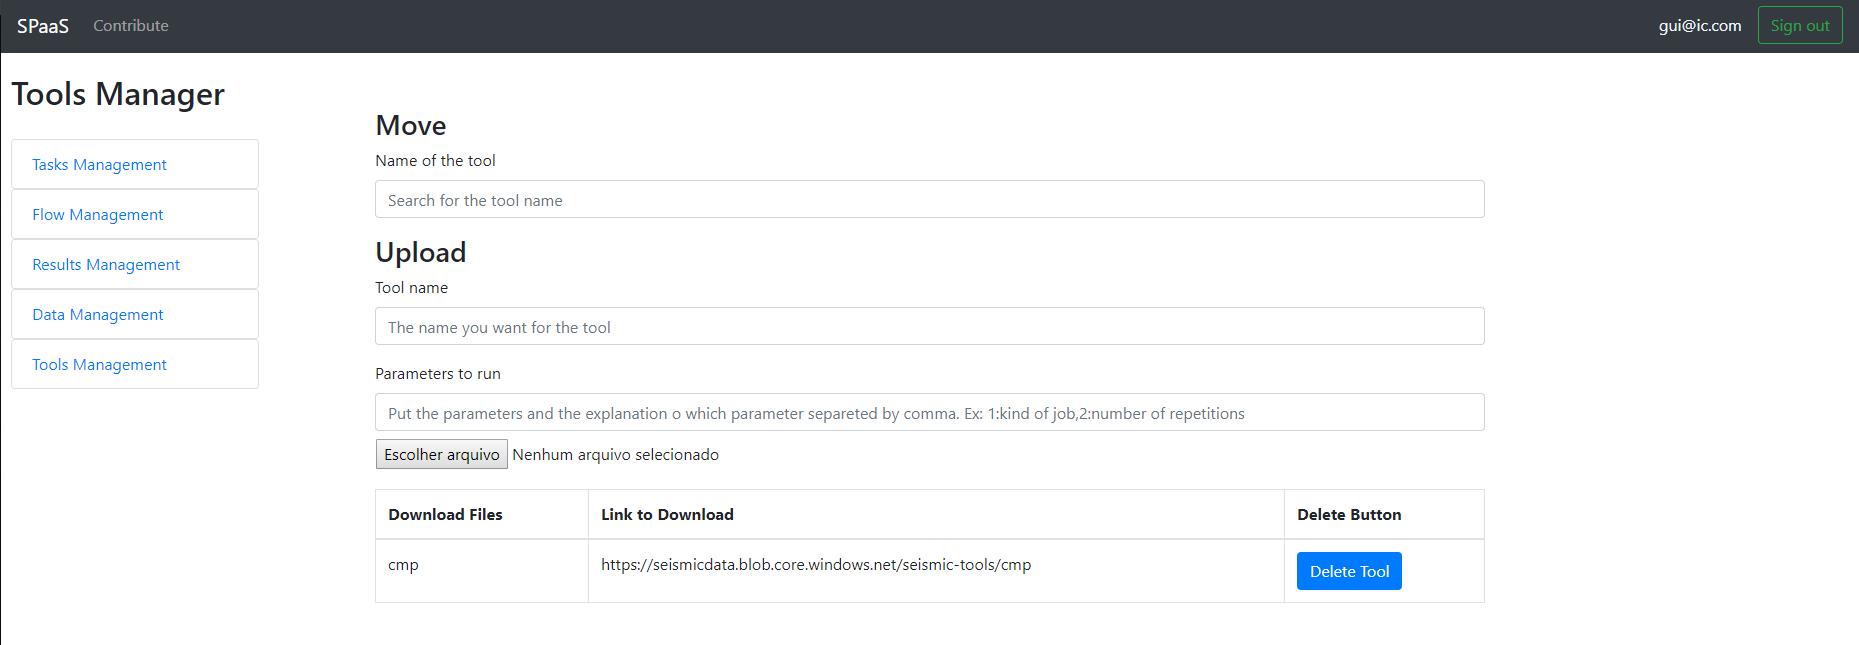
\includegraphics[scale=0.3]{tools_final.eps}
  \caption{Tela final de gerenciamento de binários}
  \label{fig:finalTools}
\end{figure}

Extremamente parecida com a tela referente aos dados, a figura ~\ref{fig:finalTools} mostra a tela de gerenciamento dos binários que foram submetidos para a plataforma. Aqui também deve
ser selecionado um arquivo, um nome e quais os parâmetros necessários para a execuçãoo, juntamente com suas explicações. Assim, os parâmetros são submetidos da seguinte maneira: 1:explicação do parâmetro 1,
2:explicação do parâmetro 2, etc.

\begin{figure}[!h]
  \centering
  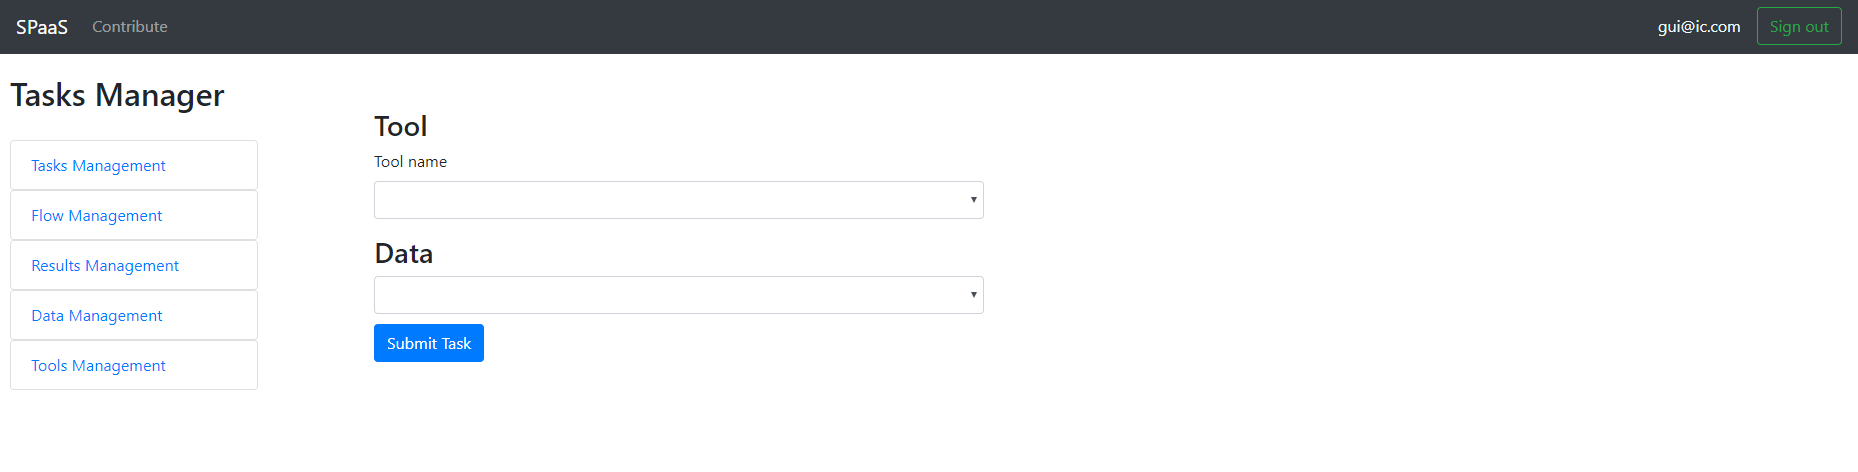
\includegraphics[scale=0.3]{task_first_final.eps}
  \caption{Tela final de gerencimento de processamentos}
  \label{fig:finalTasks}
\end{figure}

\begin{figure}[!h]
  \centering
  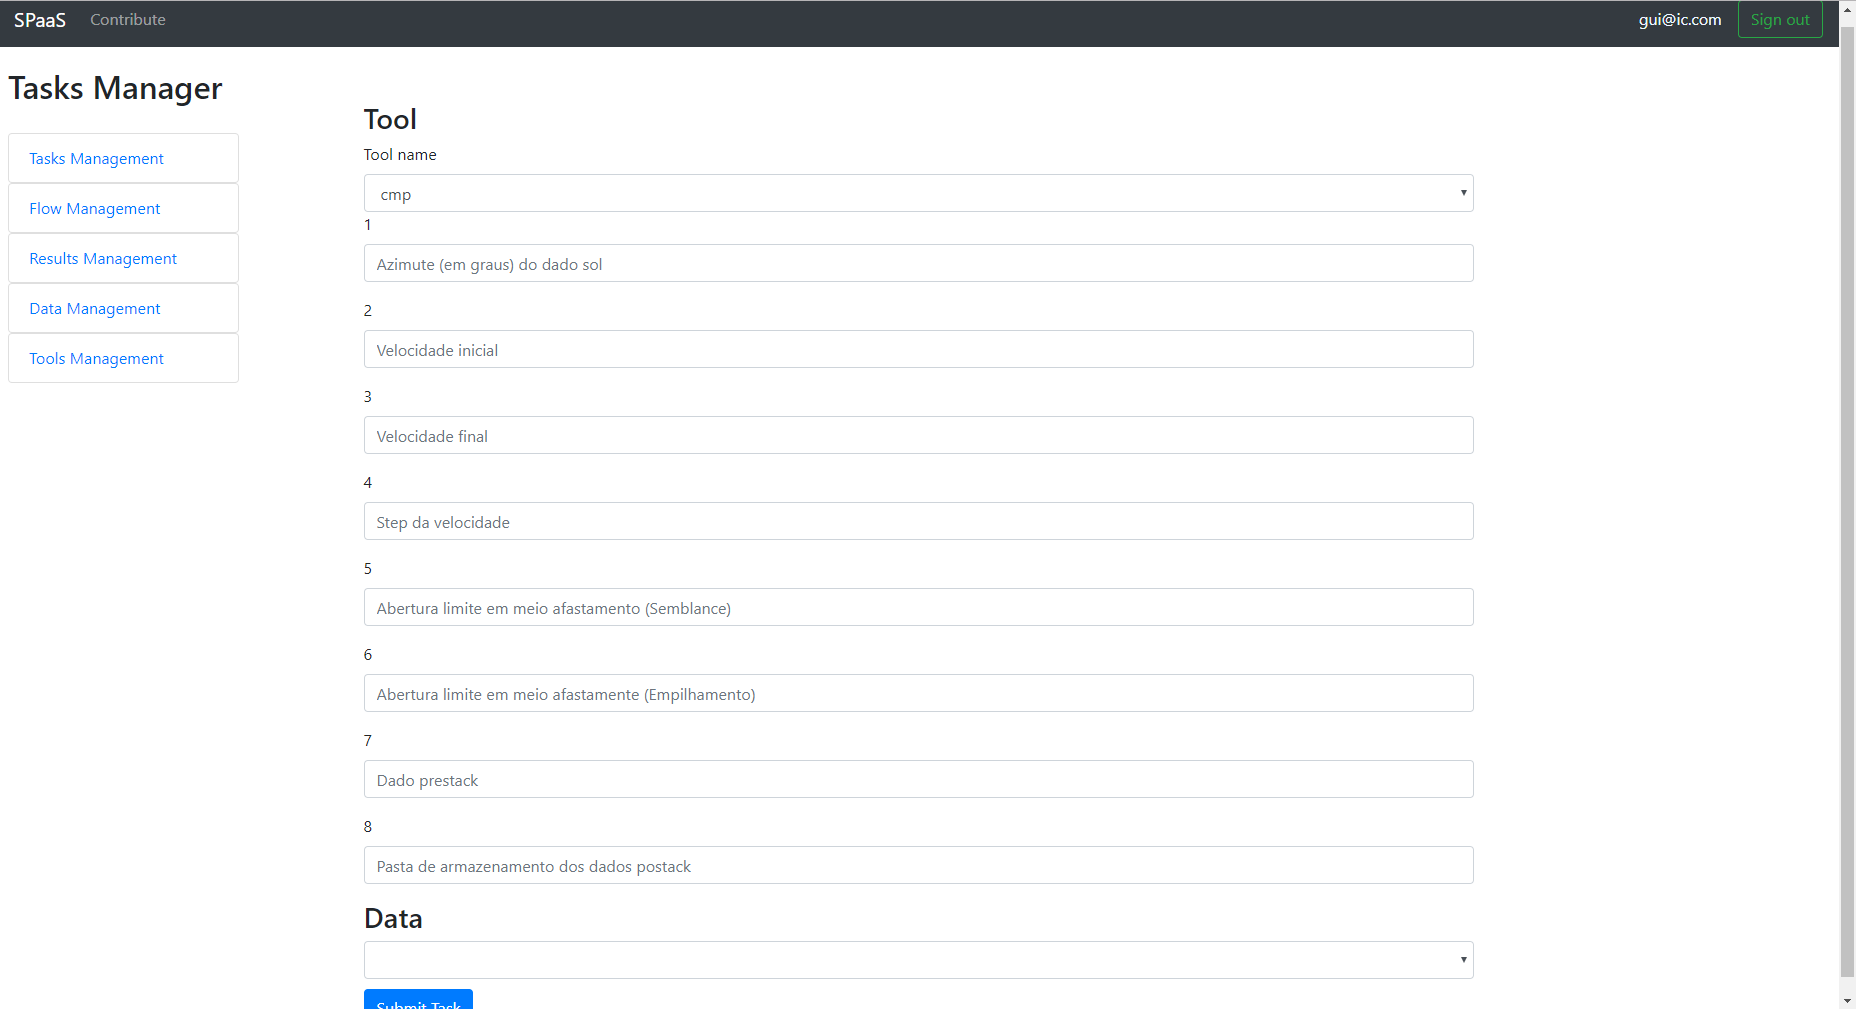
\includegraphics[scale=0.3]{task_args_final.eps}
  \caption{Tela final de processamento detalhada}
  \label{fig:finalDetailedTask}
\end{figure}

A figura ~\ref{fig:finalTasks} mostra como é a definição de um pedido de processamento que será submetido. Nesse primeiro momento, só é possível escolher um binário e o dado que serão usados, porém como mostra 
a figura ~\ref{fig:finalDetailedTask}, após selecionar o binário que será executado serão automaticamente carregados quais são os argumentes necessários para a execução com sucesso dessa tarefa. Esses argumentos
foram submetidos juntamente com o binário na tela representada pela figura ~\ref{fig:finalTools}.

\begin{figure}[!h]
  \centering
  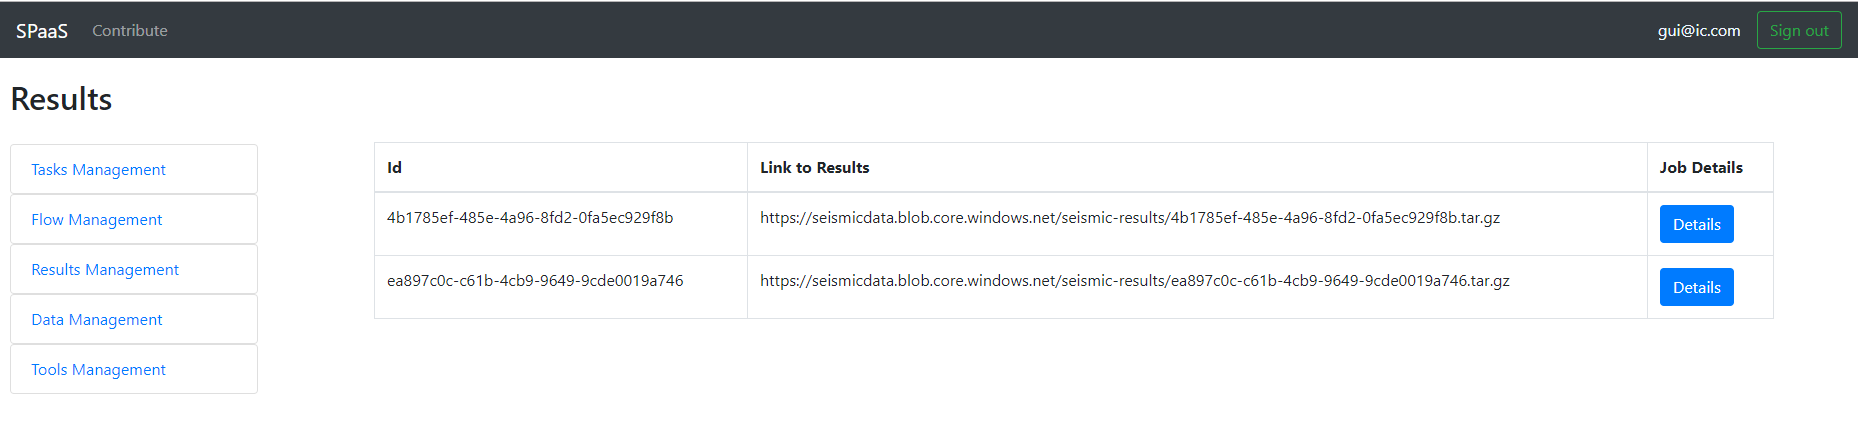
\includegraphics[scale=0.3]{results_final.eps}
  \caption{Tela final de gerenciamento de resultados}
  \label{fig:finalResults}
\end{figure}

\begin{figure}[!h]
  \centering
  
\includegraphics[scale=0.6]{results_detail_final.eps}
  \caption{Tela final com detalhes do processamento nos resultados}
  \label{fig:finalResultsDetail}
\end{figure}

Na tela de resultados, representada pela figura ~\ref{fig:finalResults}, fica claro como podemos obter os resultados depois de terminados com sucesso os processamentos. Além disso, caso o usuário queira verificar 
quais foram os dados, binários e argumentos que geraram aqueles resultados, é possível através do botão de details, que gera o json com as características daquele processamento, como é possível ver na 
figura ~\ref{fig:finalResultsDetail}.


\begin{thebibliography}{99}

\bibitem{BB} B. Burns, {\it Designing Distributed Systems,} O'Reilly Media (2017).

\bibitem{BP} B. Perens et al., {\it Debian Social Contract,} (1997).

\bibitem{BORG} A. Verma, L. Pedrosa  et al., {\it Large-scale cluster management at Google with Borg,} (2015).

\bibitem{UPP} A. Verma, L. Pedrosa  et al., {\it Cloud Computing Security: A Systematic Literature Review,} (2015).

\bibitem{HPC} K. Paladugu and S. Mukka, {\it Systematic Literature Review and Survey on High Performance Computing in Cloud,} (2012).

\end{thebibliography}

\end{document}
